\section{Environment Setup} 
%\textcolor{red}{let's move this section as an appendix}
In this section, we will present the different environments used, including the programming language, code editors, and other essential tools.

\subsection{Python}
Python is a high-level, interpreted programming language renowned for its readability and simplicity. Its clear and straightforward syntax makes it a popular choice among both novice and experienced programmers. \cite{vanrossum2009python}.

\subsection{Visual Studio Code}
Visual Studio Code also known as VS code is a free open source source code that was developed by Microsoft. Developers value its wide use and high esteem for its extensive features, flexibility, and ease of use.

\section{Tools Used}
In this section, we will be showing all the tools and software we used in order to make our project work.

\subsection{OpenCV}
OpenCV, short for Open Source Computer Vision Library, is an open-source computer vision and machine learning software library. It provides a comprehensive set of functions and algorithms for image and video processing, object detection and tracking, facial recognition, and more.

\subsection{PyTesseract}
Pytesseract is a Python wrapper for Tesseract, an open-source Optical Character Recognition (OCR) engine. OCR technology allows computers to recognize and extract text from images or scanned documents. Pytesseract makes it easy to use Tesseract's OCR capabilities in Python applications including document processing, text extraction from images, automated data entry, and more.
\subsection{Transformers}
The \texttt{transformers} library by Hugging Face was utilized for implementing and fine-tuning the TrOCR model. This library provides state-of-the-art pre-trained models for natural language processing and computer vision tasks, with seamless integration into the PyTorch ecosystem. It was crucial for loading pre-trained TrOCR architectures and adapting them to our medical label dataset.

\subsection{Optuna Library}
\texttt{Optuna} is an automatic hyperparameter optimization framework, and it was used to optimize the performance of Tesseract OCR and TrOCR by efficiently searching through hyperparameter spaces. Its flexibility and support for pruning underperforming trials contributed significantly to reducing training time and improving model accuracy.

\subsection{Deap}
The \texttt{DEAP} (Distributed Evolutionary Algorithms in Python) library was used as an alternative to Optuna for hyperparameter optimization. It leverages genetic algorithms to evolve hyperparameter sets over multiple generations, allowing exploration of a wider range of configurations, especially when search spaces are large or non-convex.

\subsection{Pandas}
\texttt{Pandas} was extensively used for handling CSV files containing image labels, ground truth text, and evaluation metrics. It facilitated the preprocessing, merging, and filtering of tabular data across various stages of the OCR pipeline, including dataset preparation and result analysis.

\subsection{Numpy}
\texttt{NumPy} provided efficient numerical operations for data manipulation, particularly in pre-processing image arrays, computing evaluation metrics such as accuracy and BCER (Bad Character Error Rate), and handling multi-dimensional arrays during training and evaluation phases.

\subsection{PyTorch}
\texttt{PyTorch} served as the primary deep learning framework for training and fine-tuning both TrOCR and EasyOCR models. Its dynamic computation graph and extensive support for GPU acceleration enabled efficient experimentation, training, and deployment of custom OCR models on medical labels.

\section{Published Paper}
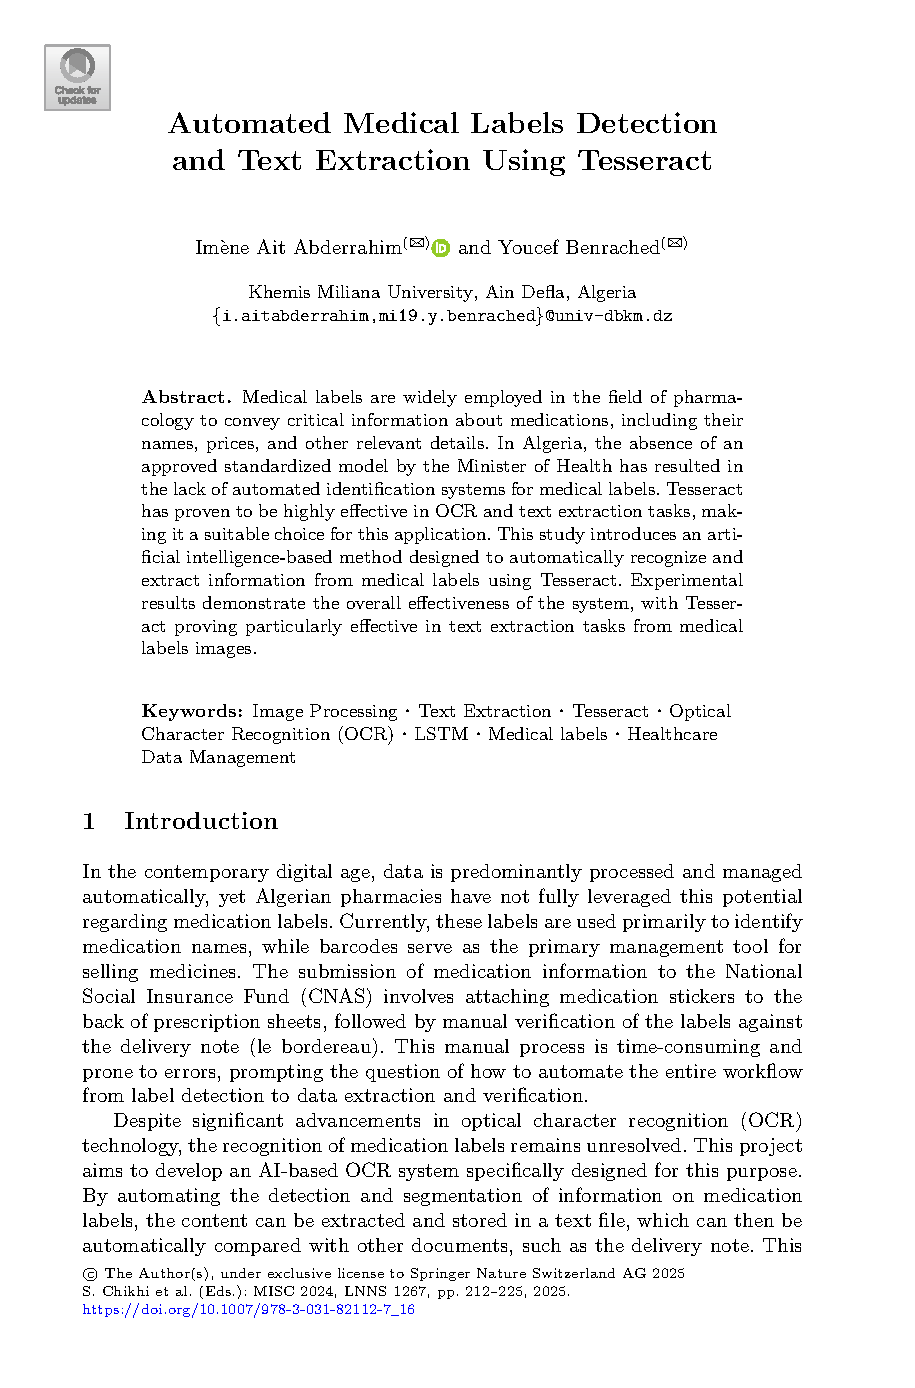
\includepdf[pages=-]{MISC2024.pdf}
